\newcommand{\NWtarget}[2]{\hypertarget{#1}{#2}}
\newcommand{\NWlink}[2]{\hyperlink{#1}{#2}}
\newcommand{\NWtxtMacroDefBy}{Fragment defined by}
\newcommand{\NWtxtMacroRefIn}{Fragment referenced in}
\newcommand{\NWtxtMacroNoRef}{Fragment never referenced}
\newcommand{\NWtxtDefBy}{Defined by}
\newcommand{\NWtxtRefIn}{Referenced in}
\newcommand{\NWtxtNoRef}{Not referenced}
\newcommand{\NWtxtFileDefBy}{File defined by}
\newcommand{\NWtxtIdentsUsed}{Uses:}
\newcommand{\NWtxtIdentsNotUsed}{Never used}
\newcommand{\NWtxtIdentsDefed}{Defines:}
\newcommand{\NWsep}{${\diamond}$}
\newcommand{\NWnotglobal}{(not defined globally)}
\newcommand{\NWuseHyperlinks}{}
\documentclass[12pt]{report}
\usepackage[a4paper, left=2cm, right=2cm, top=2cm]{geometry}
%\usepackage[text={16cm,24cm}]{geometry}
\usepackage{marginnote}


% https://stackoverflow.com/a/27243065/505306
% Making caption font smaller on figures and tables.
\usepackage{caption}
\captionsetup{font=footnotesize}

% Forcing line-breaks in url's
% https://tex.stackexchange.com/questions/3033/forcing-linebreaks-in-url
\usepackage[hyphens]{url}

%-------------------------------------------------------------------------------
%\usepackage[left,pagewise]{lineno}
%\linenumbers
\usepackage[framemethod=TikZ]{mdframed}
\usepackage{wrapfig}
\usepackage{amsthm}
\usepackage{amsfonts}
\usepackage{minted}
% ------------------------------------------------------------------------------
\usepackage[toc,page]{appendix}

%-------------------------------------------------------------------------------
%https://tex.stackexchange.com/a/278199/17858
% For aligning itemize environments to left
\usepackage{enumitem}
\mdfsetup{%
   middlelinecolor=red,
   middlelinewidth=0pt,
   roundcorner=10pt}

\mdfdefinestyle{MyFrame}{%
    linecolor=black,
    outerlinewidth=0.1pt,
    roundcorner=0pt,
    innertopmargin=14pt,
    innerbottommargin=4pt,
    innerrightmargin=4pt,
    innerleftmargin=4pt,
        leftmargin = 4pt,
        rightmargin = 4pt,
    %backgroundcolor=gray!50!white}
     }
     
%-------------------------------------------------------------------------------

\definecolor{theocol}{RGB}{255, 222, 228}
\newtheorem{theo}{Theorem}
\newenvironment{ftheo}
  {\begin{mdframed}[style=MyFrame,nobreak=true, backgroundcolor=theocol]\begin{theo}}
  {\end{theo}\end{mdframed}}


\definecolor{lemcol}{RGB}{226, 255, 220}
\newtheorem{lem}{Lemma}
\newenvironment{flem}
  {\begin{mdframed}[style=MyFrame,nobreak=true, backgroundcolor=lemcol]\begin{lem}}
  {\end{lem}\end{mdframed}}

\definecolor{corcol}{RGB}{227, 227, 227}
\newtheorem{cor}{Corollary}
\newenvironment{fcor}
  {\begin{mdframed}[style=MyFrame,nobreak=true, backgroundcolor=corcol]\begin{cor}}
  {\end{cor}\end{mdframed}}

\definecolor{propcol}{RGB}{227, 227, 227}
\newtheorem{prop}{Proposition}
\newenvironment{fprop}
  {\begin{mdframed}[style=MyFrame,nobreak=true, backgroundcolor=propcol]\begin{prop}}
  {\end{prop}\end{mdframed}}

\definecolor{notecol}{RGB}{255, 152, 149  }
\newenvironment{note}
  {\begin{mdframed}[style=MyFrame,nobreak=true, backgroundcolor=notecol]}
  {\end{mdframed}}

\usepackage{enumitem}

%-------------------------------------------------------------------------------
% https://tex.stackexchange.com/q/2291/17858
% if you want to create a new list from scratch
\newlist{alphalist}{enumerate}{1}
% in that case, at least label must be specified using \setlist
\setlist[alphalist,1]{label=\textbf{\Alph*.}}

%--------------------------------------------------------------------------------
\usepackage[english]{babel}
%\setlength{\voffset}{-0.75in}
\setlength{\headsep}{5pt}

%-------------------------------------------------------------------------------
\usepackage{blindtext}
\usepackage{lipsum}
\usepackage{textcomp}

%-------------------------------------------------------------------------------
\usepackage{asymptote}
\usepackage{asypictureB}
\usepackage{filecontents}
\usepackage{parskip} 
\usepackage{tocloft}
\usepackage{graphicx}                             % Include images into pdf document 
\usepackage{tikz}                                 % Useful for the circled command. Don't remove!
\usepackage{multicol}                             % For lists in two or more columns

\usepackage[nokwfunc, ruled]{algorithm2e}
\newcommand\mycommfont[1]{\footnotesize\ttfamily\textcolor{blue}{#1}}
\SetCommentSty{mycommfont}
\SetKwComment{Comment}{$\triangleright$\ }{}
\usepackage[T1]{fontenc}
%-------------------------------------------------------------------------------
\usepackage{needspace}                % So that sections/code-blocks don't straddle two pages 
\usepackage{mathtools}
\usepackage{subfig}
\usepackage{etoolbox}
\usepackage{color}
\usepackage{pifont}
\setlength{\parindent}{20pt}
% For italicizing quotes: https://tex.stackexchange.com/a/288556/17858

%-------------------------------------------------------------------------------
\usepackage[utf8]{inputenc}
\usepackage{csquotes}
\renewcommand{\mkbegdispquote}[2]{\itshape}

%-------------------------------------------------------------------------------
% Convenience commands
\newcommand*\circled[1]{\tikz[baseline=(char.base)]{\node[shape=circle,draw,inner sep=2pt] (char) {#1};}}
\providecommand{\myceil}[1]{\left \lceil #1 \right \rceil }	% Ceil function
\providecommand{\myfloor}[1]{\left \lfloor #1 \right \rfloor }	% Floor function\renewcommand{\labelitemi}{\tiny$\blacksquare$}	
\newcommand\given[1][]{\:#1\vert\:}                             % for drawing the conditional probability `|` sign neatly.
\newcommand\RR{\mathbb{R}}					% Set of reals numbers
\newcommand\CC{\mathbb{C}}					% Set of complex numbers
\newcommand\ZZ{\mathbb{Z}}					% Set of integers
\newcommand\NN{\mathbb{N}}					% Set of naturals
\newcommand\rarr{\rightarrow}					% Rightarrow
\newcommand\larr{\leftarrow}					% Leftarrow
\newcommand\defeq{\coloneqq}					% := symbol
\renewcommand\tilde{ \: \thicksim \: }				% Sane tildas
\newmdenv[topline=false, bottomline=false, skipabove=\topsep,skipbelow=\topsep]{siderules}
%\setlength{\droptitle}{-18em}					% Eliminate the default vertical space
%\hypersetup{colorlinks=true,linkcolor=blue}


%-------------------------------------------------------------------------------
% Writing the text of a section immediately after section title
% Vedic and old british style where text immediately follows the 
% subsection number. https://tex.stackexchange.com/a/99177/17858
%\usepackage{titlesec}
%\titlespacing{\section}{0pt}{*0}{*0}
%\titlespacing{\subsection}{0pt}{*0}{*0}
%\titlespacing{\subsubsection}{0pt}{*0}{*0}
\usepackage[compact]{titlesec}
\titlespacing{\section}{0pt}{2ex}{1ex}
\titlespacing{\subsection}{0pt}{1ex}{0ex}
\titlespacing{\subsubsection}{0pt}{0.5ex}{0ex}
%\setlength{\parskip}{0.1cm} % Paragraph separation
\setlength{\parindent}{2em}

\titleformat*{\section}{\Huge\bfseries}
\titleformat{\subsection}[runin]{\normalfont\Large\bfseries}{\thesubsection}{0.5em}{}
\titleformat*{\subsubsection}{\Large\bfseries}
%{\normalfont\huge\bfseries}{\sectiontitlename\ \thesection:}{1em}{} 
%% Custom Literate Proof Commands:
%\newcommand{\newchunk}[2]{\section{#2}\label{sec:#1}\quad}
\newcommand{\newchunk}{\subsection{}\quad}
\newcommand{\refchunk}[1]{\ref{sec:#1}}
%\newcommand{\sect}[1]{\section{#1}\quad} 
%-------------------------------------------------------------------------------
% For centeriing the titile
% https://tex.stackexchange.com/a/290449/17858
\usepackage{titling}
\renewcommand\maketitlehooka{\null\mbox{}\vfill}
\renewcommand\maketitlehookd{\vfill\null}

%-------------------------------------------------------------------------------
% To express an idea in a crunchy way.
\newcommand{\crunchy}[1]{\lbrack{} \large \textit{#1} \normalsize \rbrack} 
%-------------------------------------------------------------------------------
\makeatletter
\def\@makechapterhead#1{%
  %%%%\vspace*{50\p@}% %%% removed!
  {\parindent \z@ \raggedright \normalfont
    \ifnum \c@secnumdepth >\m@ne
        \huge \bfseries \@chapapp\space \thechapter
        \par\nobreak
        \vskip 20\p@
    \fi
    \interlinepenalty\@M
    \Huge \bfseries #1\par\nobreak
    \vskip 40\p@
  }}
\def\@makeschapterhead#1{%
  %%%%%\vspace*{50\p@}% %%% removed!
  {\parindent \z@ \raggedright
    \normalfont
    \interlinepenalty\@M
    \Huge \bfseries  #1\par\nobreak
    \vskip 40\p@
  }}
\makeatother


\usepackage{fancyhdr}
\usepackage{datetime}

\fancyhf{}
\fancyfoot[L]{\today\ \currenttime}
\pagestyle{fancy}

% https://tex.stackexchange.com/a/458876/17858 rounded
% pink rectangles around an inline word
\newcommand{\sticker}[1]{\tikz[baseline=(X.base)]\node [draw=red,fill=pink!60,semithick,rectangle,inner sep=2pt, rounded corners=3pt] (X) { {\footnotesize \color{red} #1}};}


\newif\ifshowcode
\showcodetrue
\usepackage{latexsym}
\usepackage{listings}
\usepackage{color}
\definecolor{linkcolor}{rgb}{0, 0, 0.7}

\usepackage[%
backref,%
raiselinks,%
pdfhighlight=/O,%
pagebackref,%
hyperfigures,%
breaklinks,%
colorlinks,%
pdfpagemode=None,%
pdfstartview=FitBH,%
linkcolor={linkcolor},%
anchorcolor={linkcolor},%
citecolor={linkcolor},%
filecolor={linkcolor},%
menucolor={linkcolor},%
pagecolor={linkcolor},%
urlcolor={linkcolor}%
]{hyperref}


% % %-------------------------------------------------------------------------------
% % %https://tex.stackexchange.com/a/141662/17858
% % %reset numbering of theorems, lemmas and corollaries every chapter 
% \usepackage{chngcntr}
% \counterwithin*{theo}{chapter} 
% \counterwithin*{lem}{chapter} 
% \counterwithin*{cor}{chapter} 


%% For making lualatex work with asymptote
%% ripped from https://tex.stackexchange.com/a/376412/17858
\usepackage{ifluatex}
\ifluatex
\makeatletter
\def\asy@input@graphic{%
  \ifASYinline
    \IfFileExists{"\AsyFile.tex"}{%
      \catcode`:=12\relax
      \@@input"\AsyFile.tex"\relax
    }{%
      \PackageWarning{asymptote}{file `\AsyFile.tex' not found}%
    }%
  \else
    \IfFileExists{"\AsyFile.\AsyExtension"}{%
      \ifASYattach
        \ifASYPDF
          \IfFileExists{"\AsyFile+0.pdf"}{%
            \setbox\ASYbox=\hbox{\includegraphics[hiresbb]{\AsyFile+0.pdf}}%
          }{%
            \setbox\ASYbox=\hbox{\includegraphics[hiresbb]{\AsyFile.pdf}}%
          }%
        \else
          \setbox\ASYbox=\hbox{\includegraphics[hiresbb]{\AsyFile.eps}}%
        \fi
        \textattachfile{\AsyFile.\AsyExtension}{\phantom{\copy\ASYbox}}%
        \vskip-\ht\ASYbox
        \indent
        \box\ASYbox
      \else
        \ifASYPDF
          \includegraphics[hiresbb]{\AsyFile.pdf}%
        \else
          \includegraphics[hiresbb]{\AsyFile.eps}%
        \fi
      \fi
    }{%
      \IfFileExists{"\AsyFile.tex"}{%
        \catcode`:=12
        \@@input"\AsyFile.tex"\relax
      }{%
        \PackageWarning{asymptote}{%
          file `\AsyFile.\AsyExtension' not found%
        }%
      }%
    }%
  \fi
}
\makeatother
\fi

%%%%%%%%%%%%%%%%%%%%%%%%%%%%%%%%%%%%%%%%%%%%%%%%%%%%%%%%%%%%%%%%
%% for setting program fonts
%% As recommended by http://nepsweb.co.uk/docs/progfonts.pdf
%% He recommends bera mono. 
%%\usepackage[scaled]{beramono}
%%\usepackage[T1]{fontenc}

%% I liked txtt also. 
\renewcommand{\ttdefault}{txtt}
\usepackage{tocloft}
\renewcommand{\cftpartfont}{\LARGE\itshape} % Part title in Huge Italic font
\usepackage{hyperref}
\usepackage{etoolbox}
\usepackage{upquote}

\author{Gaurish Telang}
\begin{document}

\begin{titlepage}
	\centering
        {\Huge Experimental Analyses of Heuristics for Horsefly-type Problems\\}
        \vspace{20mm}
        {\Large Gaurish Telang}
\end{titlepage}
% This gives the titlepage the page number of 1, 
% making it easier to navigate with a pdfviewer
% such as zathura, which seems to only be able 
% to understand page-numbers beginning from 1. 
\setcounter{page}{2} 

% For global table of contents
\setcounter{tocdepth}{1}
\tableofcontents
\addtocontents{toc}{~\hfill\textbf{Page}\par}

\part{Overview}
\chapter{Descriptions of Problems}
\label{chap:descriptions-of-problems}


\begin{figure}[H]
  \centering

  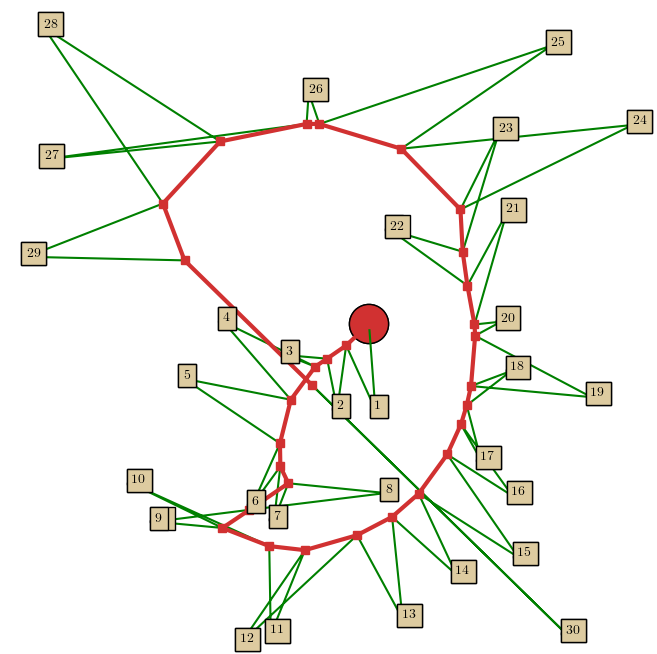
\includegraphics[width=8cm]{../webs/docs/prelim_example_phi5.png}
  \caption{An Example of a classic Horsefly tour with $\varphi=5$. The red dot
    indicates the initial position of the horse and fly, given as part of 
    the input. The ordering of sites shown has been computed with a greedy 
    algorithm which will be described later}
  \label{fig:prelim-example}
\end{figure}


The Horsefly problem is a generalization of the well-known Euclidean Traveling Salesman Problem.
In the most basic version of the Horsefly problem (which we call \textbf{``Classic Horsefly''}), we are given a set of sites, the
initial position of a truck(horse) with a drone(fly) mounted on top, and the speed of the
drone-speed $\varphi$. \footnote{ The speed of the truck is always assumed to be 1 in any of the problem 
  variations we will be considering in this report.} \footnote{ $\varphi$ is also called the ``speed ratio''.}. 

The goal is to compute a tour for both the truck and the drone to deliver package to sites
as quickly as possible. For delivery, a drone must pick up a package from the
truck, fly to the site and come back to the truck to pick up the next package for
delivery to another site. \footnote{ The drone is assumed to be able to carry at most one package at a time }
Both the truck and drone must coordinate their motions to minimize the time it takes for
all the sites to get their packages. Figure \ref{fig:prelim-example} gives an example of such a tour
computed using a greedy heuristic for $\varphi=5$.


This suite of programs implement several experimental heuristics, to solve the above NP-hard
problem and some of its variations approximately. In this short chapter, we give a description 
of the problem variations that we will be tackling. Each of the problems, has a corresponding chapter 
in Part 2, where these heuristics are described and implemented. We also give comparative analyses of 
their experimental performance on various problem instances. 

\vspace{0.5cm}

\begin{description}
\item[Classic Horsefly] This problem has already described in the introduction.

\item[Segment Horsefly] In this variation, the path of the truck is restricted to that of a segment, 
  which we can consider without loss of generality to be $[0,1]$. All sites, without loss of generality 
  lie in the upper-half plane $\RR^2_{+}$. 

\item[Fixed Route Horsefly] This is the obvious generalization of Segment Horsefly, where the path
  which the truck is restricted to travel is a piece-wise linear polygonal path. 
  \footnote{More generally, the truck will be restricted to travelling on a road network, which would 
    typically be modelled as a graph embedded in the plane.} Both the initial 
  position of the truck and the drone are given. The sites to be serviced are allowed to lie anywhere in $\RR^2$. 
  Two further variations are possible in this setting, one in which the truck is allowed reversals
  and the other in which it is not. 

\item[One Horse, Two Flies] The truck is now equipped with two drones. Otherwise the setting, is exactly 
  the same as in classic horsefly. Each drone can carry only one package at a time. The drones must fly back
  and forth between the truck and the sites to deliver the packages. We allow the possibility that 
  both the drones can land at the same time and place on the truck to pick up their next package. \footnote{In reality, 
    one of the drones will have to wait for a small amount of time while the other is retrieving its package. 
    In a more realisting model, we would need to take into account this ``waiting time'' too.}

\item[Reverse Horsefly] In this model, each site (not the truck!) is equipped with a drone, which fly 
  \textit{towards} the truck to pick up their packages. We need to coordinate the motion of the truck 
  and drone so that the time it takes for the last drone to pick up its package (the ``makespan'') is 
  minimized. 

\item[Bounded Distance Horsefly] In most real-world scenarios, the drone will not be able to (or allowed to) go more than
  a certain distance $R$ from the truck. Thus with the same settings as the classic horsefly, but with the added 
  constraint of the drone and the truck never being more than a distance $R$ from the truck, how would one 
  compute the truck and drone paths to minimize the makespan of the deliveries? 

\item[Watchman Horsefly] In place of the TSP, we generalize the Watchman route problem here. 
  \footnote{ although abstractly, the Watchman route problem can be viewed as a kind of TSP}
  We are given as input a simple polygon and the initial position of a truck and a drone. The drone has 
  a camera mounted on top which is assumed to have $360^{\circ}$ vision. Both the truck and drone can move, 
  but the drone can move at most euclidean distance \footnote{The version where instead geodesic distance is 
    considered is also interesting} $R$ from the truck. 

  We want every point in the polygon to be seen by the drone at least once. The goal is to minimize the time it 
  takes for the drone to be able to see every point in the simple polygon. In other words, we want to minimize
  the time it takes for the drone (moving in coordinattion with the truck) to patrol the entire polygon. 
  
\end{description}

\chapter{Installation and Use}

To run these programs you will need to install Docker, an open-source containerization program that is easily installable on 
  Windows 10\footnote{You might need to turn on virtualization explicitly in your BIOS, after installing Docker 
  as I needed to while setting Docker up on Windows. Here is a snapshot of an image when turning on Intel's 
  virtualization technology through the BIOS: 
\url{https://images.techhive.com/images/article/2015/09/virtualbox_vt-x_amd-v_error04_phoenix-100612961-large.idge.jpg}}, MacOS, and almost any 
  GNU/Linux distribution. For a quick introduction to containerization, watch the first two minutes of 
  \url{https://youtu.be/_dfLOzuIg2o}

The nice thing about Docker is that it makes it easy to run softwares on different OS'es portably and neatly side-steps the 
dependency hell problem (\url{https://en.wikipedia.org/wiki/Dependency_hell}.) The headache of installing different library 
dependencies correctly on different machines running different OS'es, is replaced \textbf{only} by learning how to 
install Docker and to set up an X-windows connection between the host OS and an instantiated container running GNU/Linux. 

\begin{alphalist}
\item \crunchy{Get Docker} For installation instrutions watch
  \begin{description}
    \item[GNU/Linux]  \url{https://youtu.be/KCckWweNSrM}
    \item[Windows]    \url{https://youtu.be/ymlWt1MqURY}
    \item[MacOS]      \url{https://youtu.be/MU8HUVlJTEY}
  \end{description}

\item \crunchy{Download customized Ubuntu image} \verb| docker pull gtelang/ubuntu_customized| \footnote{The customized Ubuntu image is approximately
  7 GB which contains all the libraries (e.g. CGAL, VTK, numpy, and matplotlib) that I typically use to run 
  my research codes portably.On my home internet connection downloading this Ubuntu-image typically takes about 5 minutes. }
\item \crunchy{Clone repository} \verb|git clone gtelang/horseflies_literate.git|
\item \crunchy{Mount and Launch} 
\begin{description}
\item[For GNU/Linux] Open up your favorite terminal emulator, such xterm and then
{\small
\begin{itemize}
   \item Copy to clipboard the output of \verb|xauth list|
   \item \verb|cd horseflies_literate|
   \item \verb|docker run -it --name horsefly_container --net=host -e DISPLAY -v /tmp/.X11-unix -v `pwd`:/horseflies_mnt gtelang/ubuntu_customized|
   \item \verb|cd horseflies_mnt| 
   \item \verb|xauth add | \textit{<paste-from-clipboard>}
\end{itemize}}
\item[For Windows] I had to follow the instructions in 
      \url{https://dev.to/darksmile92/run-gui-app-in-linux-Docker-container-on-windows-host-4kde} to be 
      able to run graphical user applications
\end{description}

\item \crunchy{Run experiments} If you want to run all the experiments as described in 
  the paper again to reproduce the reported results on your machine, then run \footnote{ Allowing, of course,
  for differences between your machine's CPU and mine when it comes to reporting absolute running time}, \\
  \verb|python main.py --run-all-experiments|. 

  If you want to run a specific experiment, then run \\ \verb|python main.py --run-experiment <experiment-name>|. 

  See Index for a list of all the experiments. 

\item \crunchy{Test algorithms interactively}  If you want to test the algorithms in interactive mode 
  (where you get to select the problem-type, mouse-in the sites on a canvas, set the initial position of 
  the truck and drone and set $\varphi$), run \verb|python main.py --<problem-name>|. The
  list of problems are the same as that given in the previous chapter. The problem name consists
  of all lower-case letters with spaces replaced by hyphens. 

  Thus for instance ``Watchman Horsefly'' becomes \verb|watchman-horsefly| and ``One Horse Two Flies''
  becomes \verb|one-horse-two-flies|. 

  To interactively experiment with different algorithms for, say, the Watchman Horsefly problem , 
  type at the terminal \verb|python main.py --watchman-horsefly|
\end{alphalist}

\vspace{1cm}

If you want to delete the Ubuntu image and any associated containers run the command \footnote{the ubuntu image is 7GB afterall!}
\begin{verbatim}
 docker rm -f horsefly_container; docker rmi -f ubuntu_customized
\end{verbatim}

That's it! Happy horseflying!
\part{Programs}
\chapter{Overview of the Code Base}
NOTE: {\footnotesize The style of presentation in this chapter has been adapted from 
Chapter 2 of the Nuweb reference manual \url{http://nuweb.sourceforge.net/nuweb.pdf}}

Almost all of the code has been written in Python 2.7 and tested using the standard CPython
implementation of the language. In some cases, calls will be made to external C\texttt{++} libraries (mostly CGAL and VTK) 
using SWIG (\url{http://www.swig.org/}). This is either for speeding up a slow 
routine or to use a function that is not available in any existing Python package.

There are three principal directories 
\begin{itemize}
 \item[\texttt{webs/}] This contains the source code for the entire project written in the nuweb format along with documents (mostly images)
                       needed during the compilation of the \LaTeX{} files which will be extracted from the \texttt{.web} files. 
 \item[\texttt{src/}] This contains the source code for the entire project ``tangled'' (i.e. extracted) from the \texttt{.web} files. 
 \item[\texttt{tex/}] This contains the monolithic \texttt{horseflies.tex} extracted from the \texttt{.web} files and a bunch 
of other supporing \LaTeX{} files. It also contains the final compiled \texttt{horseflies.pdf} (the current document) which contains the 
documentation of the project, interwoven with code-chunks and cross-references between them along with the experimental results.  
\end{itemize}  

The files in \texttt{src} and \texttt{tex} should not be touched. Any editing required should 
be done to the \texttt{.web} files, which should then be weaved and tangled using the
script \texttt{weave-tangle.sh} in the \texttt{webs} directory. 

\section{The Main Files} 

\newchunk The file \verb|main.py| is the entry-point for running code. This file takes
 care of reading command-line arguments and accordingly executing the interactive
 or experimental sections of the code for the appropriate problem. This file is in the 
 top-level folder. 


\newchunk Each of the files with prefix \texttt{algos-*}  contain implmentations of 
 algorithms for one specific problem. Thus \texttt{algos-watchman-horsefly.py} 
 contains algorithms for approximately solving the Watchman Horsefly problem. 

 All such files are in the directory \texttt{src/lib/}

\newchunk Similarly, each of the files with prefix \texttt{expt-*} contain code
 for testing hypotheses regarding a problem, generating counter-examples or 
 comparing the experimental performance of the algorithm implementations 
 for each of the problems. Thus \texttt{expt-watchman-horsefly.py} contains 
 code for performing experiments related to the Watchman Horsefly problem. 

 All such files are in the directory \texttt{src/expt/}

\section{Support Files}
\newchunk These files contain common utility functions that will be useful for manipulating
 data-structures, common plotting and graphics routines for all horsefly-type 
 problems. All such files have the prefix \texttt{utils-*}

 All such files are in the directory \texttt{src/lib/}

\newchunk To automate testing of code during implementations, tests for various 
 routines across the entire code-base have been written in files with prefix
 \texttt{test-*}.  

 Each of the main files have a corresponding test file. Tests for functions in the 
 support files and experimental files have all been implemented in the files 
 \texttt{test-utilities.py} and \texttt{test-experiments.py} respectively.  

 All such files are in the directory \texttt{src/test/}\chapter{Classic Horsefly}
\label{chap:classic-horsefly}


\chapter{Segment Horsefly}
\label{chap:segment-horsefly}\chapter{Fixed Route Horsefly}
\label{chap:fixed-route-horsefly}\chapter{One Horse, Two Flies}
\label{chap:one-horse-two-flies}
\chapter{Reverse Horsefly}
\label{chap:reverse-horsefly}\chapter{Watchman Horsefly}
\label{watchman-horsefly}




\begin{appendices}
\chapter{Index of Files}

\chapter{Index of Fragments}
None.

\chapter{Index of Identifiers}
 
\chapter{Man-page for \texttt{main.py}}
\end{appendices}

\end{document}
